%Klassediagram af programdesign (solution domain): Dette klassediagram skal værebindeledet mellem kravspecifikation og program. Klasserne skal indeholde væsent-lige attributter og operationer med typer, s˚aledes at det fremg˚ar hvordan de væ-sentlige begreber modelleres og samtidigt skal diagrammet give et overblik overprogramdesign.OBS: Klassediagrammet m˚a ikke genereres ud fra Java-kode. Klassediagrammetskal modelleres ved hjælp af et af de værktøjer nævnt if forlæsningen, fx. UMLet2,VisualParadigm3osv.
\subsection{Class Diagram of Program Design}
The class diagram can be seen in \autoref{fig:ClassDiagram}.
\begin{figure}[H]
    \centering
    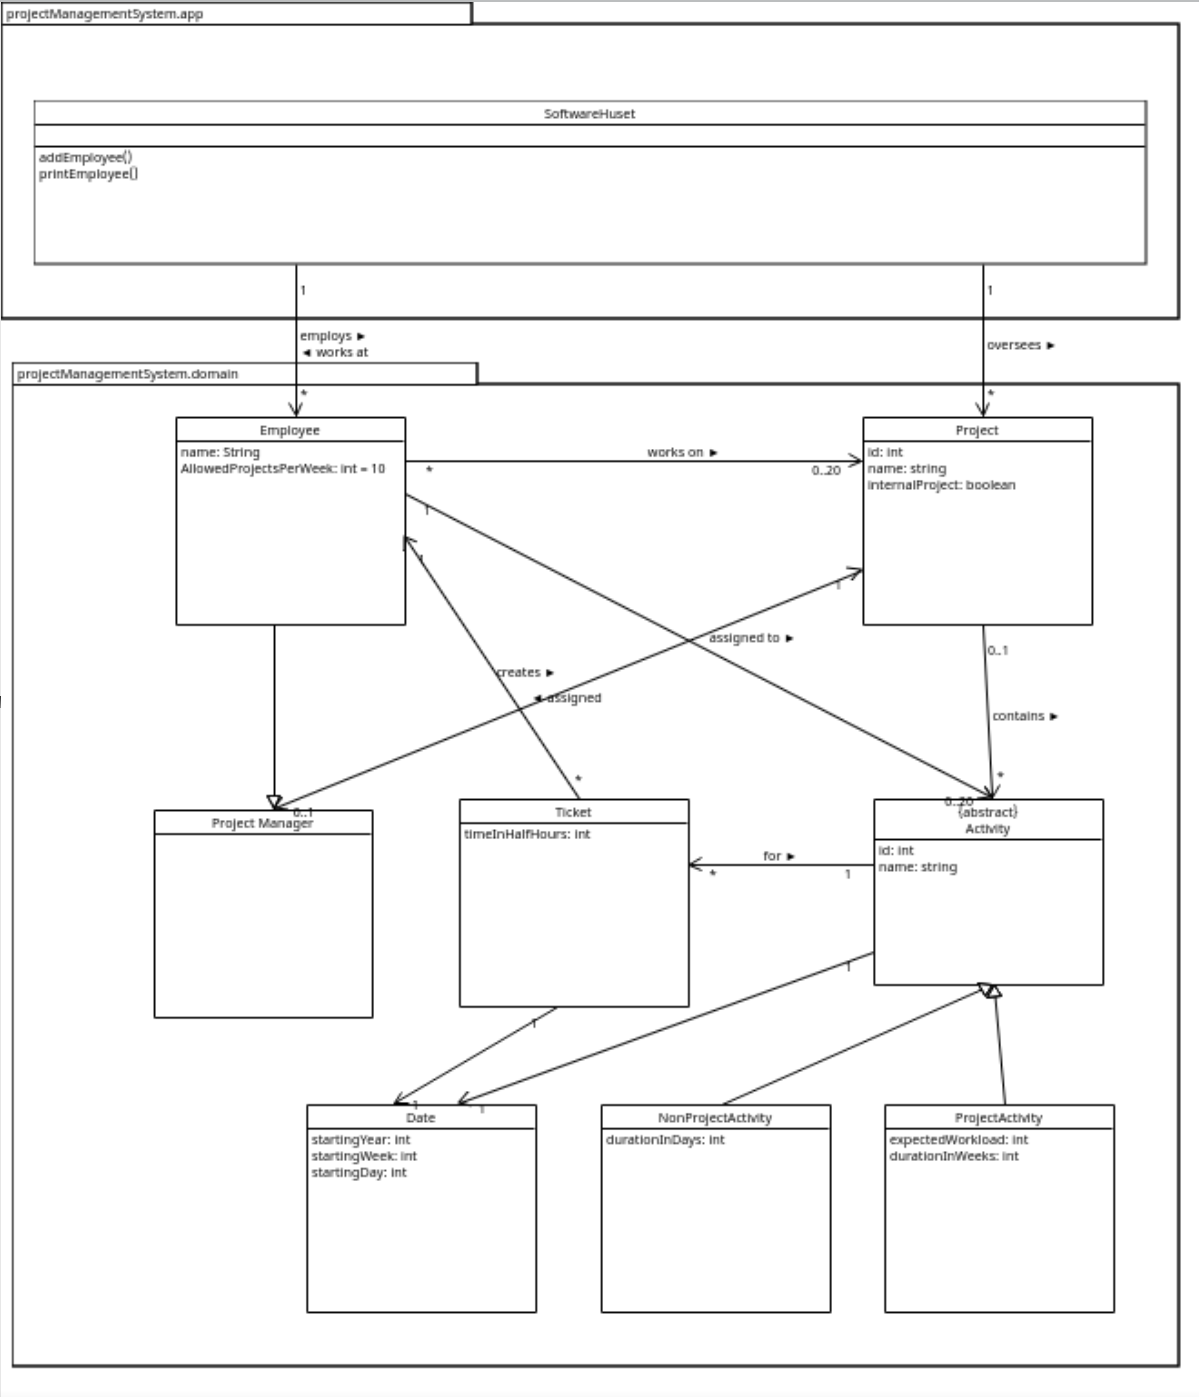
\includegraphics[width=\linewidth]{figures/ClassDiagram1.png}
    \caption{Class diagram}
    \label{fig:ClassDiagram}
\end{figure}


%Sekvensdiagrammer: Dette afsnit indeholder sekvensdiagrammer for de use casesfra afsnit 1d, s˚aledes at læseren f˚a et overblik over hvordan programmet bør udføredisse scenarier som tilhører til disse use cases. Der skal være sekvensdiagrammertil to use cases til hver gruppemedlem (et sekvensdiagram til hver hoved- ogalternative scenarier af hver use case).
\subsection{Sequence Diagrams}
This section contains sequence diagrams for all 10 Cucumber features found in section \ref{cucumber}.

\subsubsection*{Feature 1: Login to the system}
%1. Login to the system.


\subsubsection*{Feature 2: Create a new project}%Max 1
%2. Create a new project with a name and an ID.


\subsubsection*{Feature 3: Create non-project activity}
%3. Create a non-project activity and give it a starting date and expected duration.


\subsubsection*{Feature 4: Register time spent on activity}
%4. Register time spent working on an activity on a given day, even if I havent been specifically assigned to that activity.


\subsubsection*{Feature 5: Set project manager for a project}%Max 2
%5. Set myself as project manager - for a project that doesn't have a manager - and set starting week, duration and expected workload.


\subsubsection*{Feature 6: Edit project}
%6. Edit the project.


\subsubsection*{Feature 7: Create project activity}
%7. Create an activity in said project with starting date, duration and expected workload.


\subsubsection*{Feature 8: Assign an employee to a project activity}
%8. Assign an employee to an activity in said project.


\subsubsection*{Feature 9: Check available employees}
%9. View the employees who are available to be assigned during the time designated for an activity.


\subsubsection*{Feature 10: Create project report}
%10. Create a detailed report of my project, which showcases relevant metrics for evaluation.




%Afsnittet afsluttes med en kort diskussion hvor der, for eksempel, gøres rede for de valg derer truffet. Afsnittet kan ogs˚a omtale valg af algoritmer og datastrukturer.Slidserne i uge 6 anbefaler en process som kan bruges til at lave programdesign.
\subsection{Discussion}


